\documentclass[Thesis]{subfiles}

% ---------------------------------------------------------------------------
\begin{document}
	
\pagenumbering{arabic}
\chapter{Introduction}

\vspace{-1.2cm}
\begin{tabular}{lr}
	\begin{minipage}{0.4\textwidth}
		\mbox{}
	\end{minipage}
	\begin{minipage}[t]{0.57\textwidth}
		\singlespacing
		\footnotesize
		"\textit{Fra la precisa descrizione di un fatto del passato e l'accurata previsione del futuro non c'\`{e} alcuna relazione, ma \`{e} ovvio che l'una tende a rendere pi\`{u} credibile l'altra.} $[$There is no connection between the precise description of past events and the accurate prediction of the future, but obviously the one lends credibility to the other$]$."
\begin{flushright}
		Tiziano Terzani (\citeyear{terzani1995indovino}), \textit{Un indovino mi disse}
\end{flushright}	
	\end{minipage}
	\vspace{1cm}	
\end{tabular}

\noindent Mortality modelling and forecasting have a long history in demographic and actuarial analysis. The origin of mortality modelling as a research field, and of demography as a scientific discipline, is generally identified with the figure of John Graunt. In \citeyear{graunt1662natural}, Graunt presented his \textit{Natural and Political Observations Made upon the Bills of Mortality} to the Royal Society of London, the treatise that is considered to have laid the foundations of modern demography. Since then, many efforts have been devoted to the search for an encompassing model that could describe the age-pattern of human mortality accurately and parsimoniously. 

Mortality forecasting is a relatively more recent endeavour. Although forecasts of mortality can be traced back at least to the beginning of the twentieth century, research on mortality forecasting flourished during the last three decades. A new ensemble of mortality models, characterised by a common reliance on sound statistical and stochastic methods, has been proposed with the explicit goal of forecasting longevity improvements. 

Life expectancy at birth, which measures the average number of years that a newborn will live \cite[if age-specific mortality rates remain constant over time,][]{preston2001demogr}, has been increasing worldwide since around 1800 \citep{riley2001rising}. The rise of human longevity is undoubtedly one of the most remarkable achievements of modern societies \citep{oeppen2002broken}; however, improvements in survival as well as declines in fertility have generated a global process of population ageing. According to the United Nations, populations in virtually all countries and areas of the world are growing older, with persons over age 65 being the fastest-growing age group \citep{United2019wpp}. As a result, public and private sectors face increasing challenges to provide adequate pension products and elderly health care.

The difficulty of funding retirement products has become so pervasive and pressing in our ageing societies that the financial industry has coined the term "longevity risk" when referring to this issue. Longevity risk is defined as the risk that retirees could live longer (on average) than expected. From a financial perspective, this is a risk whenever an institution provides payments depending on how long individuals are going to live \citep{blake2014sharing}: if many (more than average) people live longer than their estimated life expectancy, the institution will face greater monetary outflows than its planned reserves. Small differences between the realized and previously projected lifespans of pensioners become highly magnified in the financial market: the potential size of the global longevity risk market has recently been estimated to lie between \$60 and \$80 trillion \citep{michaelson2014strategy}. As such, the need for innovative models that can predict the future course of mortality more accurately than previous approaches is evident and timely; according to \cite{janssen2018advances} and \cite{bengtsson2019intro}, this need is greater than ever before.  

The main goal of this dissertation is to propose innovative statistical methods that can provide novel insights into the analysis and forecasting of human mortality. Demographic and actuarial studies of mortality typically focus on whole populations, or large sub-populations, where only a handful of covariates are known (generally age, time and sex). Similarly, the methods proposed in this dissertation are primarily developed for studying mortality at the aggregate level.

This introductory Chapter is organised as follows. Section \ref{Sec:Ch1sec1} introduces the structure and the source of data that we use throughout this dissertation, as well as the main functions and measures typically employed in mortality studies. Sections \ref{Sec:Ch1sec2} and \ref{Sec:Ch1sec3} review the main historical developments and contributions to the fields of mortality modelling and forecasting. The specific aims of the thesis are presented in Section \ref{Sec:Ch1sec4}. From Section \ref{Sec:Ch1sec5} to \ref{Sec:Ch1sec9}, we provide a short introduction to the Chapters of this dissertation. Section \ref{Sec:Ch1sec10} discusses the methodologies presented in this thesis and their related results, and it outlines some possible directions for future work. Finally, Section \ref{Sec:Ch1sec11} provides the links and information for using the routines and reproducing the results of this dissertation.

\section{Preliminaries}\label{Sec:Ch1sec1}

\subsection*{Mortality data}\label{Subsec:Ch1subsec1.1}
An understanding of the data that are typically employed in mortality studies is a necessary first step to performing research on mortality modelling and forecasting. This study starts by describing the general structure of mortality data, as well as the specific source of data that we use throughout this dissertation. 
 
The graphical illustration of mortality data is a convenient way to understand its structure. The principal tool for visualizing this type of data is the Lexis diagram \citep{lexis1875einleitung}, a graph that depicts the life histories of different individuals through so-called life-lines. A Lexis diagram displays the three main dimensions along which mortality is primarily measured, namely age, period (i.e.~calendar year) and (birth) cohort. These dimensions are related by the well-known identity $cohort = period - age$. In a Lexis diagram, age and period are represented on the $y$- and $x$-axis, respectively, while cohort corresponds to left-to-right diagonals.

The left panel of Figure \ref{Fig:Ch1Lexis} shows a simplified Lexis diagram for a population closed to migration, in which several life-lines are shown for two different birth cohorts. All life-lines start from the $x$-axis, and they move along diagonals with slope equal to one as time passes and individuals age. The lines stop once the individuals experience death, which is represented by a red point in the graph. Censoring and truncation are not considered in this example.

\begin{figure}[!ht]
	\begin{center}
		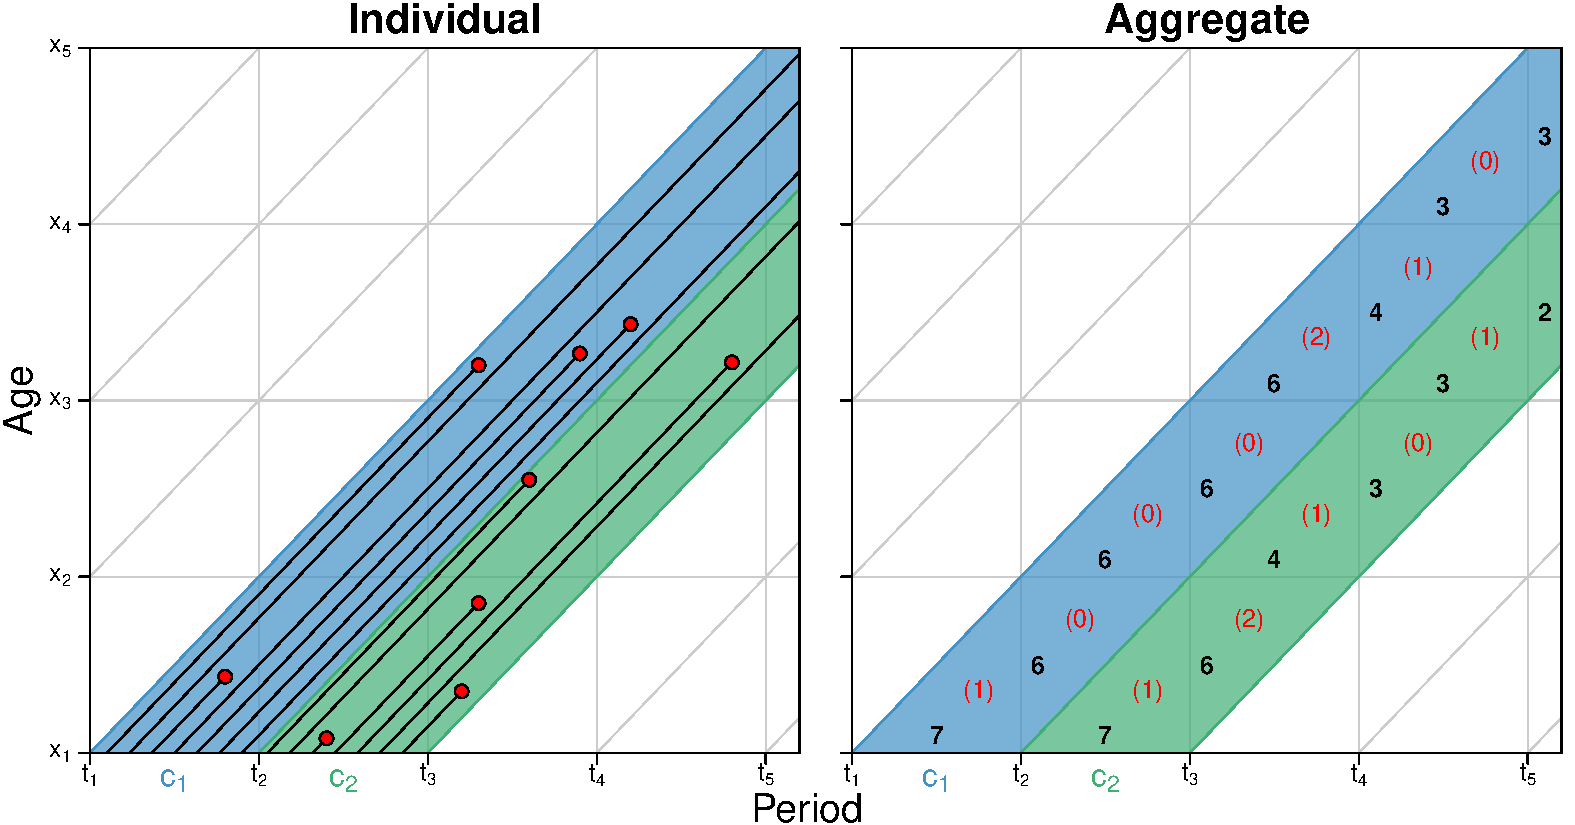
\includegraphics[scale=0.60]{./Ch1/F0.pdf}
		\caption{Two simplified Lexis diagrams that illustrate individual life-lines (left panel) and aggregate mortality data (right panel) for the cohorts $c_1$ and $c_2$ (blue and green areas, respectively). In the left panel, red points represent the death of the individual. The age and period dimensions correspond to the $y$- and $x$-axis, respectively.\\
		\textit{Source}: Own elaborations, inspired by Figure 1.1 in \cite{camarda2008smoothing}.}\label{Fig:Ch1Lexis}
	\end{center}
\end{figure} 

When the research question concerns the analysis of mortality patterns and developments of rather large populations, exact life-lines for millions of individuals are rarely known. It is therefore customary and convenient to group together individual life-lines within the same lower and upper triangles of the diagram. This allows one to efficiently summarize death and population data at the aggregate level by age, period and cohort. The right panel of Figure \ref{Fig:Ch1Lexis} shows a Lexis diagram in which aggregate mortality data have been computed from the left panel. 

Clearly, the availability of aggregate mortality data is paramount for the purpose of this dissertation. Traditional sources of such datasets are censuses, official vital statistics and population registries, which are routinely collected in several developed countries. In the year 2000, the University of California at Berkeley (United States) and the Max Planck Institute for Demographic Research (Rostock, Germany) initiated a far-sighted collaborative project called the \citeauthor{HMD} (HMD, \citeyear{HMD}), with the aim of providing researchers, policy makers and others with a unique source of accurate, homogenised and comparable national data on birth, death and population counts for several countries. Today, the HMD provides free access to detailed, consistent and high quality mortality data for 41 different countries or areas via the Internet \citep{barbieri2015data,wilmoth2019protocol}. The database has gained increasing attention during recent years, becoming one of the main sources of data for mortality studies: up to August 2019, almost 3500 journal articles have been published relying on the HMD\footnote{source: \url{https://www.mortality.org/Public/HMD-Publist.pdf}}.

Data in this dissertation are thus uniquely retrieved from the HMD. For all the manuscripts in this thesis except Chapter \ref{Ch5}, we perform mortality analysis on the traditional age-period perspective depicted in Figure \ref{Fig:Ch1Lexis}. As such, we derive from the HMD observed death counts $y_{x,t}$ and central exposures to the risk of death $e_{x,t}$ at age $x$ and time $t$. Let bold capital and small letters denote matrices and vectors, respectively.  Data are arranged into two matrices $\bm{Y} = (y_{x,t})$ and $\bm{E} = (e_{x,t})$, each of dimensions $m \times n$, where: (i) rows are classified by $m$ single ages at death, $\bm{x}'=\left[x_1,\dots,x_m\right]$, and (ii) columns are classified by $n$ single years, $\bm{t}'=\left[t_1,\dots,t_n\right]$. Visually, the matrices can be shown as follows:
%
\begin{equation}\label{Eq:Ch1YEmat}
\bm{Y} = \begin{bmatrix}
y_{x_1,t_1} & y_{x_1,t_2} & \dots & y_{x_1,t_n} \\
y_{x_2,t_1} & y_{x_2,t_2} & \dots & y_{x_2,t_n} \\
\vdots & \vdots & \ddots & \vdots \\
y_{x_m,t_1} & y_{x_m,t_2} & \dots & y_{x_m,t_n}
\end{bmatrix} \, , \qquad \bm{E} = \begin{bmatrix}
e_{x_1,t_1} & e_{x_1,t_2} & \dots & e_{x_1,t_n} \\
e_{x_2,t_1} & e_{x_2,t_2} & \dots & e_{x_2,t_n} \\
\vdots & \vdots & \ddots & \vdots \\
e_{x_m,t_1} & e_{x_m,t_2} & \dots & e_{x_m,t_n}
\end{bmatrix} \, . \notag
\end{equation}
%

In Chapter \ref{Ch5}, we shift the focus of the analysis to the age-cohort perspective. The structure of the available mortality data is different and characterized by unobserved data for some elements of $\bm{Y}$ and $\bm{E}$. A full description of the structure of age-cohort mortality data is provided in Section \ref{Sec:Ch5sec2} of Chapter \ref{Ch5}.

The matrices $\bm{Y}$ and $\bm{E}$ allow us to compute one of the principal measures of mortality, namely central death rates, which are often denoted age-specific mortality rates. Specifically, the rate $m_{x,t}$ at age $x$ and time $t$ is computed by dividing the corresponding death counts by exposures, i.e.~$m_{x,t} = y_{x,t} / e_{x,t}$. Death rates for all ages and years can then be arranged in the matrix $\bm{M} = (m_{x,t})$. As a practical illustration, Figure \ref{Fig:Ch1Data} displays the available mortality data for Swedish females in 2017. 

\begin{figure}[!ht]
	\begin{center}
		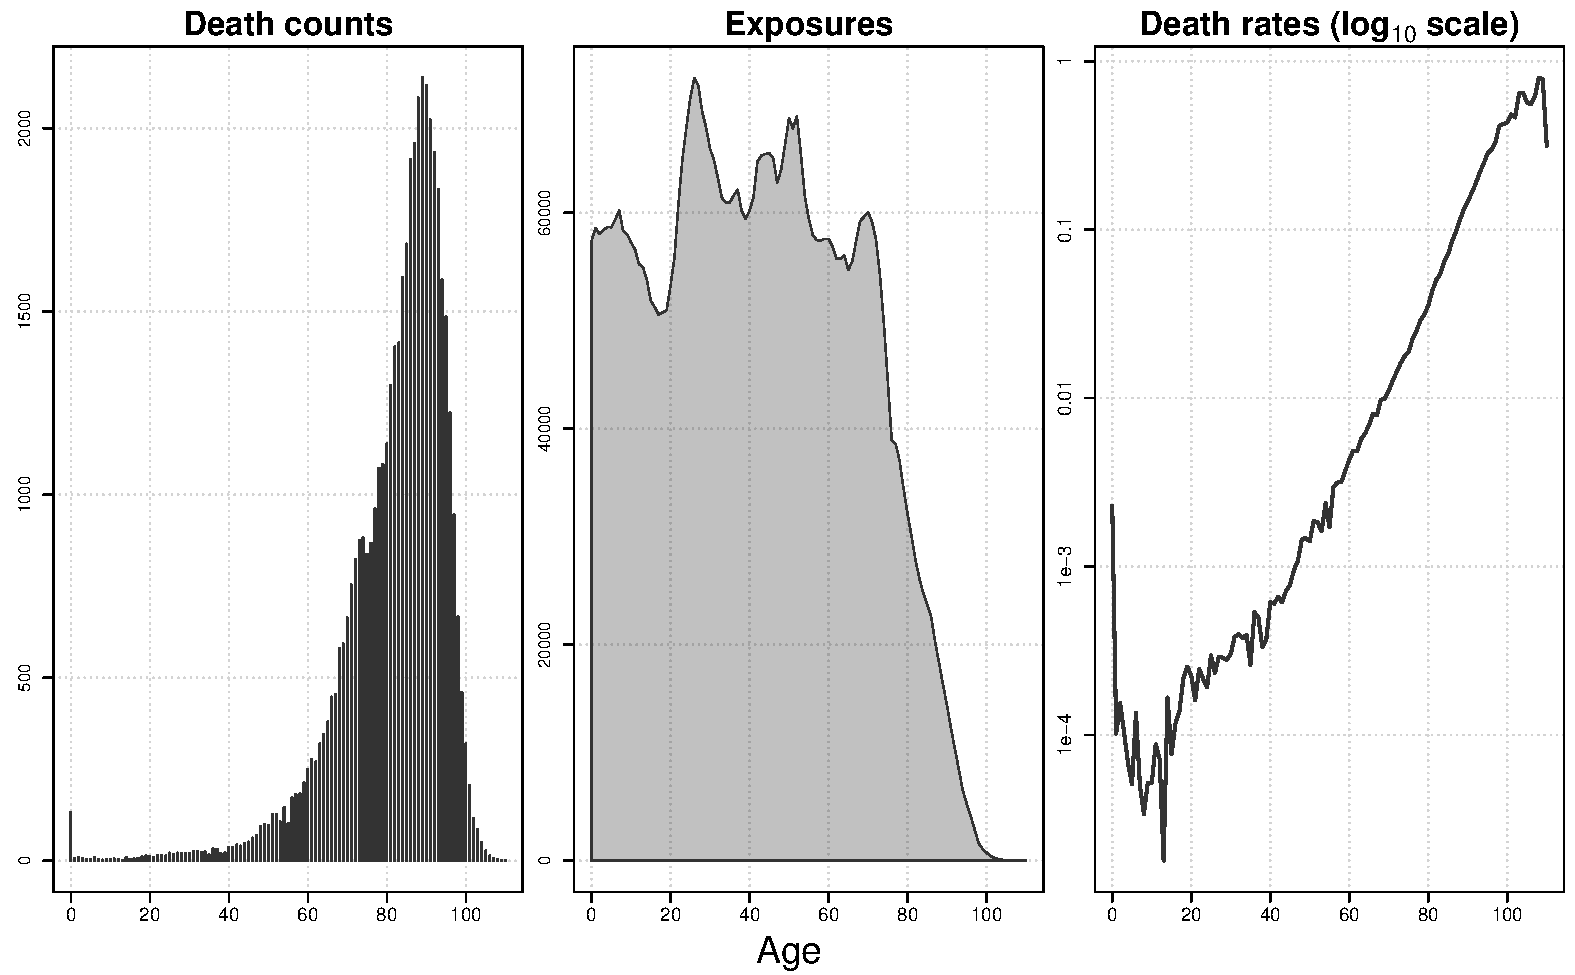
\includegraphics[scale=0.55]{./Ch1/F0b.pdf}
		\caption{Observed death counts, exposures to the risk of death and central death rates (on $\log_{10}$ scale) for Swedish females at ages 0--110+ in 2017.\\
		\textit{Source}: \cite{HMD}.}\label{Fig:Ch1Data}
	\end{center}
\end{figure} 

It is worth mentioning here that, in all manuscripts of this dissertation, we always compute death rates from the matrices $\bm{Y}$ and $\bm{E}$ instead of using the life-table death rates provided by the HMD. The former are indeed observed rates, whereas the latter are smoothed at older ages "\textit{to obtain an improved representation of the underlying mortality conditions}" \cite[][p.~34]{wilmoth2019protocol}.

\subsection*{Mortality measures and functions}\label{Subsec:Ch1subsec1.2}
Having described the structure and source of data used in this dissertation, here we introduce the measures and functions that are typically used in mortality analysis. 

Modelling and forecasting human mortality is a branch of demography that is closely intertwined with the analysis of survival data in statistics. We therefore present the measures and functions employed in the study of human mortality linking the terminologies used in survival analysis \cite[derived from][]{klein2003survival} with those used in demography \cite[derived from][]{preston2001demogr}.

Survival analysis focuses on the study of durations until the occurrence of a specific event of interest. For the purposes of this dissertation, the event of interest is death, although it could be any other event, such as marriage, conception, onset of a disease and so forth. The duration until the specified event is denoted with the random variable  $X$, which is typically continuous and non-negative. For the time being, let us think of $X$ as the age dimension of the mortality data just introduced, and let us temporarily drop the time (calendar year) dimension to ease notation. There are three functions that characterize the distribution of $X$: (i) the probability density function $f(x)$, which is the unconditional probability of death at age $x$, (ii) the survival function $S(x) = \Pr(X > x)$, which is the probability of an individual surviving to age $x$, and (iii) the hazard rate (function) $h(x)$, which is the instantaneous rate of death at age $x$, conditioned upon surviving to that age, or formally: 
%  
\begin{equation}\label{Eq:Ch1Hazard}
h(x) = \lim\limits_{\Delta x \rightarrow 0} \frac{\Pr \left(x \leq X < x + \Delta x \,|\, X \geq x \right)}{\Delta x} \, .
\end{equation}
%
As such, $h(x) \Delta x$ can be interpreted as the approximate probability that an individual of age $x$ dies in the next instant of time, given that she survived until $x$.

Figure \ref{Fig:Ch1Functions} shows an example of the three mortality functions of the Gompertz model, one of the most frequently employed parametric models of human mortality, which will be formally introduced in Section \ref{Sec:Ch1sec2}. For our purposes here, the graphs are useful to illustrate the properties of the three functions.  The left panel shows that the density is a non-negative function, whose area under the curve is equal to one, i.e.~$\int_{0}^{\infty}f(x)\,dx = 1$. The central panel displays the survival function, which is monotonically decreasing and bounded between 0 and 1, with $S(0)=1$ and $\lim_{x \rightarrow \infty}S(x)=0$. Finally, the right panel shows the hazard function, which is also non-negative at all ages, i.e.~$h(x)\geq0$ $\forall x$.

\begin{figure}[!ht]
	\begin{center}
	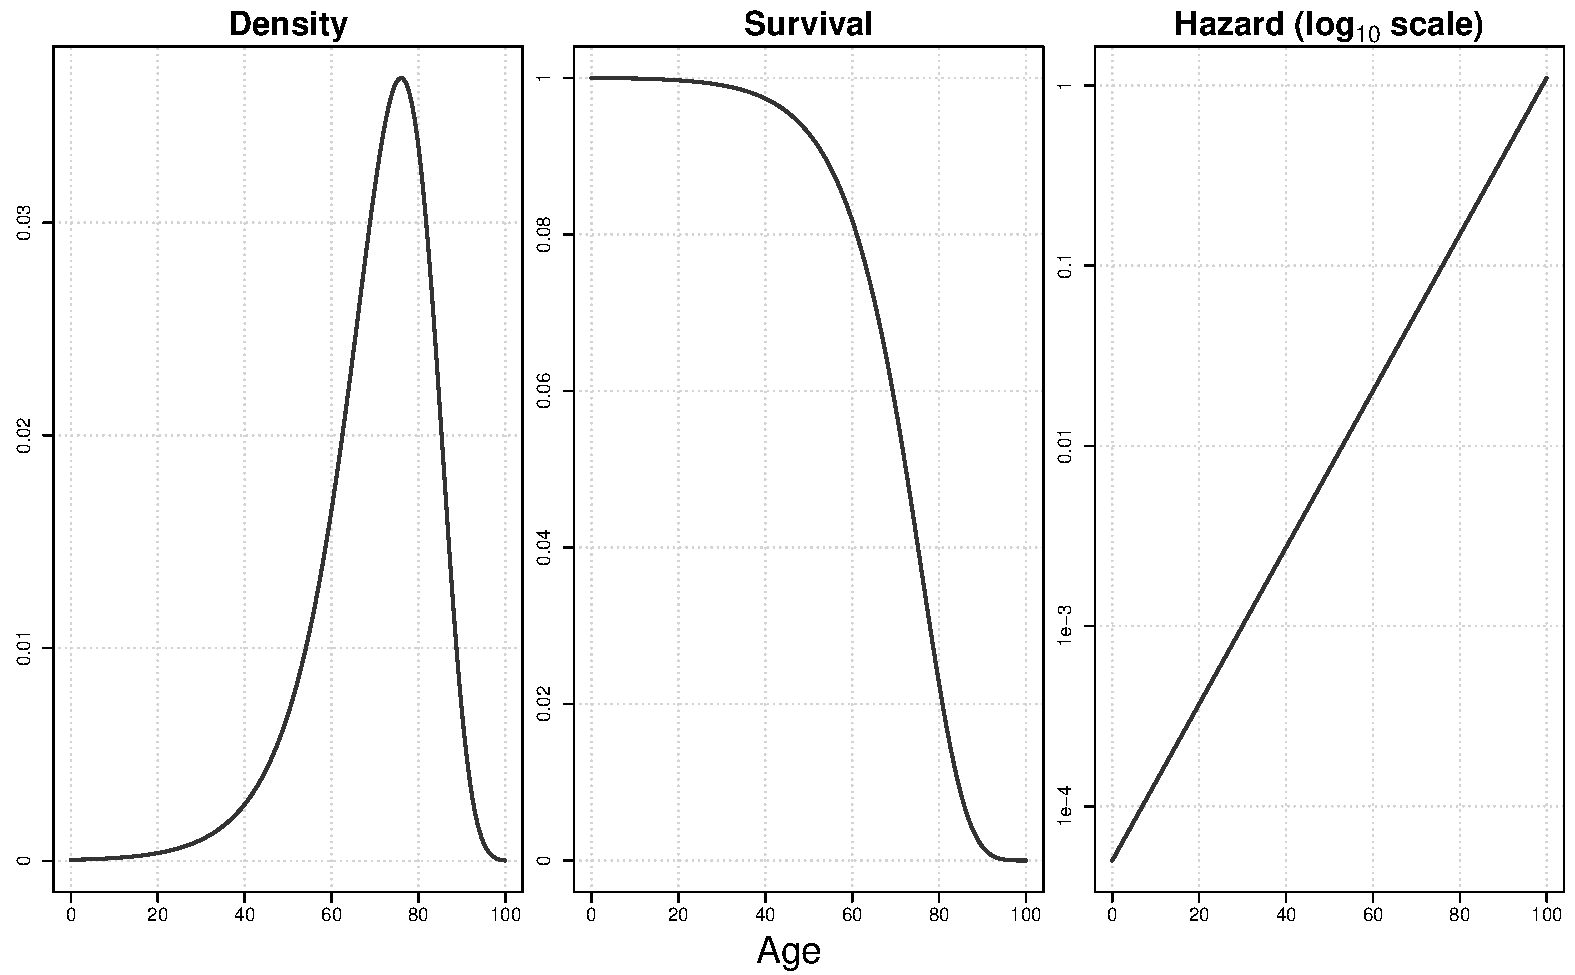
\includegraphics[scale=0.55]{./Ch1/F0c_new.pdf}
	\caption{An illustration of the density, survival and hazard functions of the Gompertz model for human mortality (cf.~Section \ref{Sec:Ch1sec2}).\\ \textit{Source}: Own elaborations.}\label{Fig:Ch1Functions}
	\end{center}
\end{figure} 
 
An important characteristic of the three mortality functions is that they are uniquely related to each other: it is possible to derive any two of them by knowing the third one, without the need of additional information. Specifically, the relationship that exists between the survival and density functions is:
%  
\begin{align}
	S(x) = \int_{x}^{\infty} f(t)\,dt \quad &\Leftrightarrow \quad f(x) = - \frac{dS(x)}{dx} \label{Eq:Ch1SurDen} \\
	\intertext{Moreover, the hazard and the survival are related by:}
	S(x) = \exp \left[-\int_{0}^{x} h(t)\,dt \right] \quad &\Leftrightarrow \quad h(x) = - \frac{d\,\ln \left[S(x)\right]}{dx} \label{Eq:Ch1SurHaz}
\end{align}
%
Combining Eq.~\eqref{Eq:Ch1SurDen} and \eqref{Eq:Ch1SurHaz} shows the complementarity of the three mortality functions, which can be expressed in terms of each other as:
%  
\begin{equation}\label{Eq:Ch1DenHazSur}
f(x) = h(x)\,S(x) \, .
\end{equation}
%

In demography, the three mortality functions are known by the notation and terminology of the life table, and although having different names, they are identical to those used in survival analysis. Let us maintain the continuous notation, before moving to the discrete formulation intrinsic to life tables. Demographers and actuaries generally denote: (i) the density function as the age-at-death distribution $d(x)$, (ii) the survival function as the probability of surviving from birth to age $x$, $\ell(x)$, and (iii) the hazard function as the force of mortality $\mu(x)$.  

Mortality is a continuous process, and the functions just introduced are well suited to capture the inherent nature of the risk of death, which constantly changes over age and time. As discussed in Section \ref{Sec:Ch1sec1}, mortality data are however collected only at particular ages and years. For this reason, the life table has long been used in mortality analysis to illustrate age-specific information about the survival and progressive extinction of a birth cohort. Given its tabular nature, a life table displays mortality functions only at particular ages (or age groups). A discrete notation is therefore appropriate to introduce the other life-table functions. 

In addition to ages $x$ and central death rates $m_x$, a life table comprises several additional columns. First, $d_x$ and $\ell_x$ (the discrete-time equivalents of $d(x)$ and $\ell(x)$) denote the number of deaths at age $x$ and the number of survivors to age $x$, respectively. Next, $a_x$ denotes the mean number of person-years lived by those dying in the interval starting with $x$; $q_x = d_x / \ell_x$ corresponds to the probability of dying in the age group $x$, and $p_x = 1 - q_x$ the complementary survival probability; $L_x$ denotes the number of person-years lived in the cohort for the age group $x$.  

The last column of the life table deserves special attention due to its extensive use in mortality analysis. This column is the life expectancy at age $x$, $\mathrm{e}_x$, which measures the average number of additional years that a survivor at age $x$ is expected to live beyond that age. Specifically, it is computed as $\mathrm{e}_x=\sum_{a=x}^{\omega}L_a / \ell_x$, where $\omega$ is the highest age attained in the life table, and it can be expressed in continuous notation as:
%  
\begin{equation}\label{Eq:Ch1LifeExp}
\mathrm{e}(x) = \frac{\int_{x}^{\infty} \ell(a)\,da}{\ell(x)} \, .
\end{equation}
%
Life expectancy at birth, $\mathrm{e}_0$, is equivalent to the mean age at death of the life-table cohort, and as such, it is a measure of central tendency of the age-at-death distribution. This measure is practically omnipresent in studies of population health, because it conveniently summarizes the mortality pattern of the population into a single number.  

However, life expectancy at birth alone does not capture all the relevant features of the distribution of deaths. Indeed, a specific mean value can originate from very different shapes of the underlying distribution. As such, scholars have recently started to go beyond the analysis of "central longevity indicators" \cite[mean, median and modal age at death,][]{cheung2005three} by analysing different summary measures of the distribution. 

In particular, the concentration of lifespan distributions in human populations, typically referred to as lifespan inequality, disparity or variability in the demographic literature, has received significant attention during recent decades.  Inequality in length of life is indeed the most fundamental of all inequalities, as every other inequality is conditional upon being alive \citep{vanraalte2018case}.

Several indices have been proposed to measure lifespan inequality, which have been shown to be highly correlated with each other \cite[see, for example,][]{wilmoth1999rectangularization,vaupel2011life,van2013perturbation,colchero2016emergence}. In this dissertation, we employ two measures of lifespan inequality: in Chapters~\ref{Ch3}-\ref{Ch5}, we use the Gini concentration index $\mathrm{G}(x)$ at age $x$, also known as Gini coefficient, which is defined as \citep{hanada1983formula,shkolnikov2003gini}:
%
\begin{equation}\label{Eq:Ch1GINI}
\mathrm{G}(x) = 1 - \frac{1}{\mathrm{e}(x)\left[\ell(x)\right]^2} \int_{x}^{\omega} \left[\ell(t)\right]^2 dt \, .
\end{equation}
%
In Chapter \ref{Ch6}, we use the average number of life years lost at age $x$ \citep{vaupel2003decomposing}:
%
\begin{equation}\label{Eq:Ch1edag}
\mathrm{e}^{\dagger}(x)= \frac{\int_{x}^{\omega} \mathrm{e}(t) \, d(t) \, dt}{\ell(x)} \, .
\end{equation}
%
Both measures have been employed to measure lifespan inequality within and between populations \cite[see, e.g.,][]{hanada1983formula,shkolnikov2003gini,smits2009length,shkolnikov2011losses,vaupel2011life,van2013perturbation,gigliarano2017longevity,aburto2018lifespan} and to evaluate mortality forecasts \citep{bohk2017lifespan,diaz2018mortality,basellini2019modelling,camarda2019smooth}. For additional details on the Gini coefficient, please refer to Section~\ref{Sec:Ch5sec4}.

Finally, two important assumptions that will be used throughout this dissertation should be mentioned here. The first is a central  assumption in demographic and actuarial analyses of mortality: the piece-wise constant hazard model. Specifically, the force of mortality $\mu_{x,t}$ is assumed to remain constant over each year of age (from age $x$ to $x+1$) and over each calendar year (from year $t$ to $t+1$). This assumption implies that: (i) $\mu_{x,t}$ approximates the force of mortality at exact age $x+\frac{1}{2}$ and exact time $t+\frac{1}{2}$, and (ii) central death rates $m_{x,t}$ are the maximum likelihood estimators (MLEs) of the force of mortality \citep{currie2016fitting}. We refer the interested reader to Chapter 4 of \cite{alho2005statistical} for the derivation of the MLE in the case of $n$ individuals with independent and identically distributed lifespans following the exponential distribution. 

Secondly, following the important work of \cite{brillinger1986biometrics}, we assume that times of birth and lifetimes in the population are stochastic, with the former following a Poisson process, and the latter being independent of each other, independent of the birth process, and corresponding to the force of mortality $\mu_{x,t}$. These assumptions imply that  the observed number of deaths $y_{x,t}$ in the population are  realizations of the random variable $Y_{x,t}$, which follows a Poisson process with expected value equal to the product of exposure and force of mortality \cite[see][p.~700]{brillinger1986biometrics}:
%
\begin{equation}\label{Eq:Ch1Poisson}
Y_{x,t} \sim \mathcal{P}(e_{x,t} \, \mu_{x,t})  \, .
\end{equation}
%
This assumption is particularly useful for estimation purposes. Let the force of mortality $\mu(\bm{\theta})_{x,t}$ be a function of age, time and a vector of parameters $\bm{\theta}$. Then, for each time period $t$, the parameters can be estimated by maximising the Poisson log-likelihood:
% 
\begin{equation}\label{Eq:Ch1PoiLogLike}
\ln \, \mathcal{L}\left(\bm{\theta}\,|\, y_{x,t}\,,e_{x,t}\, \right) \propto \sum_{x} \left[  y_{x,t} \,
\ln \left(\mu(\bm{\theta})_{x,t}\right) - e_{x,t}
\, \mu(\bm{\theta})_{x,t}  \right]  \, .
\end{equation}
% 
where the logarithm of the exposures is generally referred to as an "offset" in the context of Generalized Linear Models \cite[GLMs,][]{mccullagh1989glm}. 

In practice, the Poisson assumption implies that the relative importance of central death rates is given by the number of deaths occurring at that age. As such, the  parameters of a mortality model will be estimated to maximise the model's goodness-of-fit at those ages where most of the deaths occur. Figure~\ref{Fig:Ch1RatesWeights} displays an example of the weights and relative importance of the death rates shown in the right panel of Figure \ref{Fig:Ch1Data}. Figure~\ref{Fig:Ch1RatesWeights} clearly shows that rates at ages 80--90 are the main target of a mortality model embedded in a Poisson setting, whereas rates at young ages (excluding age 0) carry less weight.   

\begin{figure}[!ht]
	\begin{center}
		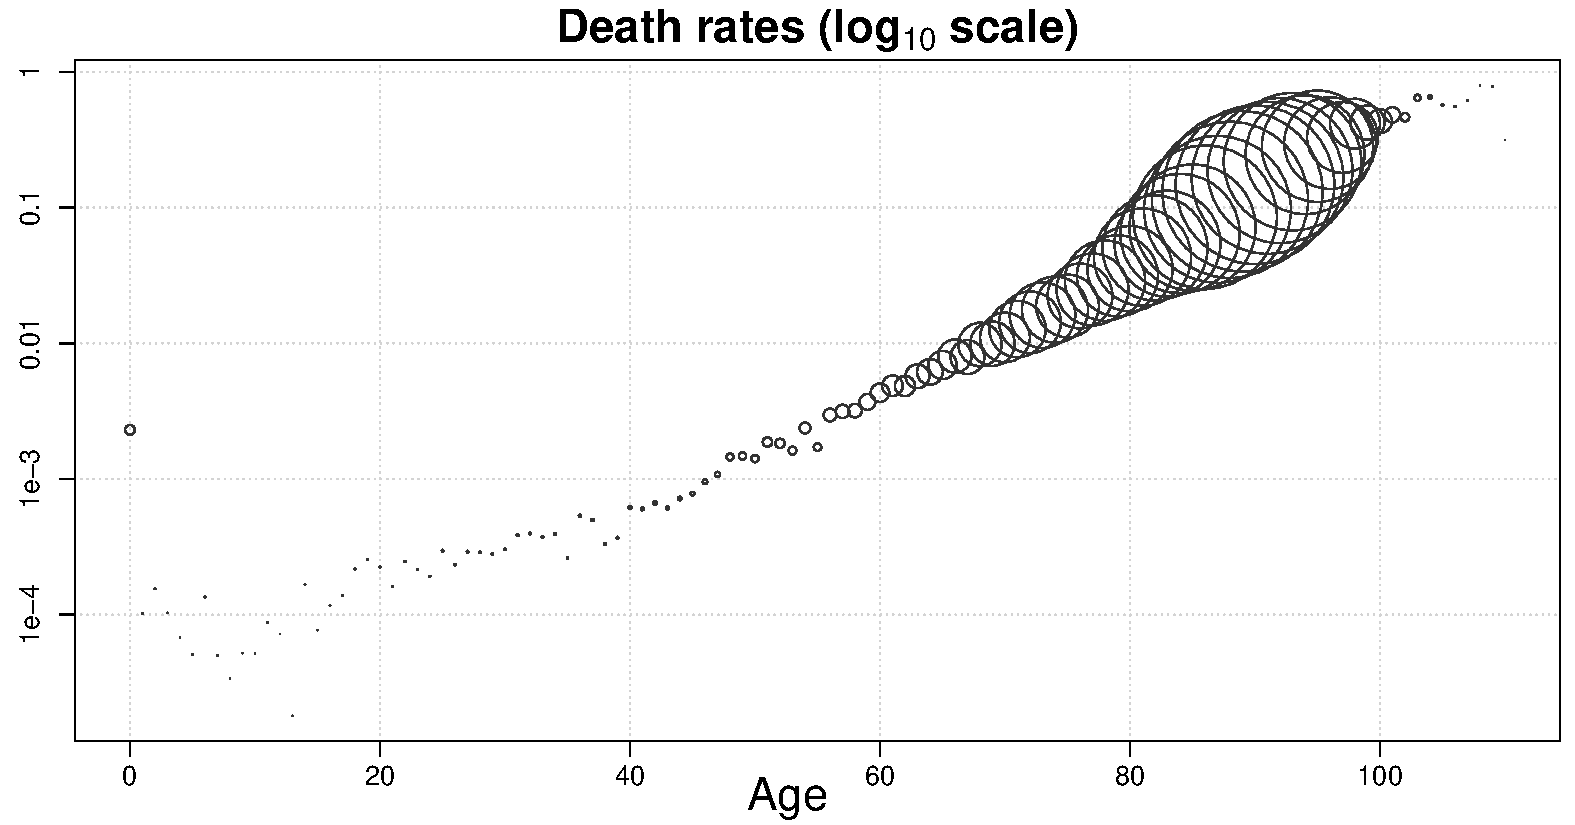
\includegraphics[scale=0.58]{./Ch1/F0d.pdf}
		\caption{Observed central death rates (on $\log_{10}$ scale) for Swedish females at ages 0--110+ in 2017. Circles are proportional to the number of deaths at the corresponding age. \\
		\textit{Source}: Own elaborations based on data from the \cite{HMD}.}\label{Fig:Ch1RatesWeights}
	\end{center}
\end{figure} 
 
\section{Mortality modelling}\label{Sec:Ch1sec2}
According to \cite{coale1983regional}, Graunt's celebrated \textit{Observations} (\citeyear{graunt1662natural}) marked the first investigation into the regularities of the mortality age-pattern. By analysing the bills of mortality in London (i.e.~weekly accounts of burials and christenings collected by various parishes), Graunt listed both the number of deaths and survivors by decades for a cohort of 100 persons, thereby introducing the first example of one of the most important tools in demography -- the life table.  

Graunt's life table was based on rather limited data, as London lacked reliable census data at the time, and the bills of mortality did not specify the ages of the deceased. Graunt complained of these deficiencies, and tried to estimate age-specific death rates indirectly by computation \citep{cole1957sketches}. For this reason, some scholars regard the work of \cite{halley1693estimate}, which was based on the more accurate register data of the city of Breslau in 1687--1691, as the first example of the modern life table. From around 1750, several other efforts were directed towards the production of life tables, which took a central place in population studies \citep{coale1983regional}.

Modern life tables expressed in single years of age comprise 500 to 1000 numbers, depending on the number of conventional columns printed. However, much of this information is redundant \citep{keyfitz1982choice}. For this reason, several efforts have been directed towards the specification of a "mortality law", i.e.~a parametric function of age, which can capture the relevant features of the age-pattern of human mortality using only a few parameters.

There are several reasons why parametric models of mortality have received so much attention during the last two centuries \citep{keyfitz1982choice,congdon1993statistical}:

\medskip
\begin{itemize}
	\item to smooth the data. Mortality rates of adjacent age groups sometimes display random fluctuations, mostly due to small sample sizes. A smooth parametric curve eliminates these uneven variations, thereby offering a more plausible representation of the underlying mortality pattern. 
	\item to describe mortality rates of several different age groups parsimoniously, by using only a few parameters. This property further allows one to derive mortality rates at any given age group (i.e.~interpolation). 
	\item to aid inferences from incomplete data. When vital registers of a population are not available, one can infer the mortality pattern by using the partial information at hand and a specific class of models (e.g.~relational models, model life tables).
	\item to facilitate comparisons of mortality. A model's parameters summarize the mortality conditions of the population analysed. As such, differences in the mortality patterns can be more easily detected by comparing the estimated parameters of different populations.
	\item to construct life tables. It is often forgotten that the life-table construction relies on a parametric model of mortality, namely the piece-wise constant hazard model (cf.~Section \ref{Sec:Ch1sec1}). 
	\item to facilitate mortality forecasting. Time-series extrapolations of the model's parameters easily allow one to obtain future mortality schedules.	
\end{itemize}
\smallskip

An early attempt to describe the age-pattern of mortality with a mathematical formula goes back to \cite{demoivre1725annuities}, who hypothesised that "the number of lives existing at any age is proportional to the number of years intercepted between the age given and the extremity of old age" \cite[][cited in \cite{smith1977mathematical}, p.~273]{demoivre1725annuities}. In terms of the mortality functions introduced in the previous Section, DeMoivre's formula can be expressed as $\ell(x)=\ell(0) \left(1-\frac{x}{\omega}\right)$,
where $\ell(0)$ is the life-table radix, and $\omega$ the maximum attainable age in the population. Without loss of generality, let the life-table radix be equal to one. The force of mortality of the one-parameter DeMoivre's law thus follows:
%
\begin{equation}
\mu(x)=\frac{1}{\omega-x} \,.
\end{equation}
%

A century later, one of the most prominent laws of mortality was contributed by Benjamin Gompertz. By analysing life tables, Gompertz observed a recurrent pattern, a geometric increase in mortality at adult ages: "this law of geometrical progression pervades, in an approximate degree, large portions of different tables of mortality" \cite[][p.~514]{gompertz1825nature}. As such, Gompertz's law of mortality can be expressed by an exponential increase of mortality with age:
%
\begin{equation}\label{Eq:Ch1Gompertz}
\mu(x)= a\, \mathrm{e}^{bx} \,,
\end{equation}
%
where the two parameters $(a,\,b) > 0$ represent the level of the force of mortality at the starting age of analysis (typically, age 30), and the rate of ageing, respectively. An example of the Gompertz law is shown in Figure~\ref{Fig:Ch1Functions} of the previous Section. The force of mortality (on a logarithmic scale) increases linearly with age, and the model's parameters $a$ and $b$ correspond to the intercept and slope of the linear model, respectively.  

The two-parameter Gompertz law has proved to be a remarkably good model for different populations and epochs \citep{forfar2004mortality}: it is an almost universal pattern that has been found to apply (over appropriate age ranges) in many countries during the last 170 years \citep{thatcher1998force}. Nevertheless, two limitations have been highlighted throughout the years: (i) the model does not include excess accident mortality at young adult ages and (ii) the model does not capture the deceleration of mortality at advanced ages \citep{manton1993forecasting,vaupel1998biodemographic}. 

The underestimation of mortality at young adult ages was identified and addressed a few decades after Gompertz by \cite{makeham1860law}, who suggested modifying Gompertz's law by adding an additional parameter to capture the constant risk of death from all causes which does not depend on age. Makeham's law of mortality is thus given by:
%
\begin{equation}\label{Eq:Ch1Make}
\mu(x)= c + a\, \mathrm{e}^{bx} \,.
\end{equation}
%

Logistic parameterizations have instead been proposed to account for the overestimation of mortality at advanced ages. These models are characterized by an upper bound for the force of mortality, which decelerates at higher ages following a mortality plateau  (i.e.~a horizontal asymptote). An early attempt in this direction was contributed by Perks, who proposed a generalization of Makeham's law because: "it was found that the Makeham curves ran much too high at the older ages" \cite[][p.~13]{perks1932some}. Nowadays, one of the most used logistic-type mortality law is the Kannisto model:
%
\begin{equation}\label{Eq:Ch1Kann}
\mu(x)= \frac{a\, \mathrm{e}^{bx}}{1 + a\, \mathrm{e}^{bx}} \,.
\end{equation}
%

Analysing thirteen countries with a sufficiently long time-series of reliable data, \cite{thatcher1998force} found that logistic curves fit the mortality pattern at old ages at least as well as, and usually better than, any other mortality models. Hence, the \cite{HMD} adopted the Kannisto model to smooth death rates above age 80 in life-table construction \cite[see][p.~34]{wilmoth2019protocol}.

All the mortality laws described thus far have been proposed to model the adult age-pattern of mortality. However, the non-monotonic shape of human mortality has long been observed and recognized by demographers and actuaries. The Danish astronomer and actuary \cite{thiele1871mathematical} contributed one of the first attempts to model the entire age-pattern of mortality: in particular, he suggested describing human mortality with three different groups that operate principally, or almost exclusively, upon childhood, middle and old ages, respectively. Formally, he suggested the following expression for the force of mortality:
%
\begin{equation}\label{Eq:Ch1Thiele}
\mu(x)=\mu_{1}(x)+\mu_{2}(x)+\mu_{3}(x)  \, ,
\end{equation}
%
where the force of mortality $\mu(x)$ at age $x$ is additively decomposed into three independent components, $\mu_{1}(x)$, $\mu_{2}(x)$, and $\mu_{3}(x)$. For mortality in childhood, $\mu_{1}(x)$, Thiele suggested a negative exponential function; for middle ages, $\mu_{2}(x)$, he suggested a negative log-parabolic curve, while for higher ages he adopted Gompertz's law. It should be further highlighted that Thiele's contribution pioneered decomposition modelling by providing one of the first examples of competing-risk hazard models. 

In recent decades, several attempts have been made towards modelling the whole pattern of mortality, all inspired by the work of Thiele. Among the most relevant contributions, \cite{siler1979competing} proposed a five-parameter model with an age-independent constant hazard for the term $\mu_{2}(x)$ in Eq.~\eqref{Eq:Ch1Thiele}. Although originally developed to portray animal mortality, the model has been used for human populations as well \cite[see, e.g.,][]{siler1983parameters,gage1993decline,canudas2005contributions,canudas2008modal,bergeron2015decomposing}. Furthermore, \cite{heligman1980age} followed Thiele's parameterization more closely and proposed an eight-parameter model to portray human mortality. \cite{kostaki1992nine}, in turn, suggested extending the Heligman-Pollard model by adding an additional parameter, which improves the fit to mortality data at younger adult ages. Moreover, \cite{de2016new} proposed a ten-parameter model that directly captures the shifting and compression dynamics of mortality changes. Finally, \cite{mazzuco2018mortality} introduced a six-parameter mixture distribution function to model the age-at-death distribution, which has been extended with the inclusion of two additional parameters by \cite{zanotto2017mixture}. For an additional short review of parametric mortality models, please refer to Subsection \ref{Subsec:Ch2subsec1.2}.   

\section{Mortality forecasting}\label{Sec:Ch1sec3}
The laws of mortality introduced in the previous Section aim to describe the age-pattern of mortality for a population at a specific point in time, or for a specific cohort of individuals. This class of mortality models is generally referred to as age-models, as the age dimension is the only explanatory variable used in the model. Another approach to modelling mortality, typically stimulated by the goal of forecasting future mortality conditions, is given by including the period dimension (i.e.~calendar years) in the modelling process. This approach has generated the class of age-period models, which are widely employed in mortality forecasting. This Section reviews the most important contributions to this field of research.

In a major review paper on demographic forecasting, \cite{booth2006demographic} distinguishes three approaches to forecasting demographic processes: extrapolation, expectation and explanation. Extrapolation is the most common approach in current demographic forecasting, and the majority of statistical offices and international organizations employ extrapolative forecasting methods \citep{booth2008mortality,stoeldraijer2013impact}. As such, here we focus on this forecasting approach.

Forecasts of mortality can be traced back at least to the beginning of the twentieth century, when English actuaries started to assess the financial effects of longevity improvements on the reserves of pension providers \citep{pollard1987projection}. For example, the London Institute of Actuaries' annuitants tables of 1924 were produced by extrapolating age-specific death probabilities observed between 1900 and 1920 to an ultimate level of mortality \cite[][pp.~183--193]{anderson1948actuarial}. 

Until the 1980s, the methods used to forecast mortality were relatively simple and involved a fair degree of subjective judgement \citep{booth2008mortality}. An excellent review of the methods in use at that time can be found in \cite{pollard1987projection}, who distinguished six types of projections by: (i) extrapolation of mortality rates at selected ages, (ii) reference to a law of mortality, (iii) reference to model life tables, (iv) reference to another more advanced population, (v) reference to an optimal life table, and (vi) causes of death.

It is however during the last three decades that mortality forecasting has prospered owing to the introduction and development of stochastic methodologies to project mortality. Much of the success enjoyed by the field has been stimulated by the seminal contribution of \cite{lee1992modeling}. Lee and Carter proposed an elegant and powerful methodology to model and forecast mortality based on a log-bilinear form for central death rates $m_{x,t}$. Formally, the Lee-Carter (LC) model can be expressed as:
\begin{equation}\label{Eq:Ch1LC}
\ln \left( m_{x,t} \right) = \alpha_x + \beta_x \kappa_t + \varepsilon_{x,t} \,,
\end{equation}
where $\alpha_x$ describes the average shape of age-specific mortality, $\beta_x$ the rate of mortality improvement at age $x$, and $\kappa_t$ the general level of mortality at time $t$. The $\varepsilon_{x,t}$ are error terms that reflect residual age-specific historical influences not captured by the model. Since the model is underdetermined, two standard constraints are used to ensure model identification, namely $\sum_{x} \beta_x = 1$ and $\sum_{t} \kappa_t = 0$. 

The LC model is today the best known and widely employed forecasting methodology. Three main reasons explain why the model has gained so much attention: (i) the functional form is not complex, as a matrix of (logged) age-specific mortality rates over time is summarized by two age-specific parameters and one time-varying index, (ii) forecasting is greatly simplified, as  mortality forecasts are derived from the projection of the single time-index, typically using a random walk model with drift, and (iii) the model is probabilistic, thereby allowing the derivation of prediction intervals of mortality rather than single deterministic point forecasts. 

Since its introduction almost thirty years ago, different limitations of the model have been highlighted, and new extensions  have been proposed to overcome them. In its original form, the LC parameters are estimated by ordinary least-squares (OLS) using singular value decomposition. In addition, the first estimates of $\hat{\kappa}_t$ are adjusted so that the fitted deaths of the model match the number of observed deaths in each year $t$. The main drawback of the OLS approach is that the errors are assumed to be homoskedastic and normally distributed, which is an unrealistic assumption for human mortality \citep{alho2000discussion}. Indeed, the logarithm of the central death rates is more variable at older than at younger ages because of the smaller number of deaths \citep{brouhns2002poisson}. To overcome this limitation, \cite{brouhns2002poisson} embedded the LC model in a Poisson setting, which is a more realistic assumption for human mortality characterized by a heteroscedastic error structure.  

A second relevant limitation of the LC model is the assumption of a constant rate of age-specific mortality improvement over time \citep{lee2001evaluating}. The assumption has proven wrong in low-mortality countries during recent decades: rates of mortality improvement have declined at infant and childhood ages, and they have increased at older ages \citep{kannisto1994reductions,vaupel1998biodemographic,wilmoth1999rectangularization}. As a result, it has been shown that the model tends to underpredict future gains in life expectancy \citep{lee2001evaluating}. To overcome this drawback, \cite{li2013extending} proposed rotating the $\beta_x$ schedule for long-term projections. This rotation captures the observed deceleration of mortality improvements at younger ages, and the acceleration at older ages.

Third, the LC fitted and forecast life tables are typically irregular, characterized by a high degree of jaggedness in the mortality age-profile. This is a consequence of the estimated model's parameters, which are generally volatile (especially the $\beta_x$ schedule). To overcome this limitation, smoothing techniques have been implemented within the LC framework. \cite{renshaw2003forecasting} suggested smoothing the estimated series of $\alpha_{x}$ and $\beta_{x}$ using parametric or non-parametric methods. \cite{hyndman2007robust} start by smoothing the observed data using a functional data approach \citep{ramsay2005FDA}. Furthermore, \cite{delwarde2007smoothing} and \cite{currie2013smoothing} proposed estimating the LC parameters by maximising a penalized log-likelihood function, which results in smooth parameter estimates and, in turn, regular forecast age-patterns.  

In addition to the already presented extensions, four other improvements of the LC model deserve mention, as they have received considerable attention and have been used in a number of publications. First, \cite{lee2001evaluating} suggested the second-step adjustment of the time-index to match exactly the observed value of life expectancy at birth $\mathrm{e}_0$. This allows one to reduce the jump-off bias, which can be particularly severe in the early years of the forecasts \citep{lee2001evaluating}. Second, \cite{booth2002applying} adjusted the time-index to reproduce the age-at-death distribution, and they further suggested a procedure to optimally restrict the fitting period in the presence of a non-linear trend in the time index. Third, \cite{renshaw2006cohort} extended the model to account for cohort effects. Fourth, \cite{hyndman2007robust} proposed employing a greater number of principal components to capture additional dimensions of change in mortality rates. In addition to this, the authors start by smoothing the observed data, and they allow for greater flexibility in the selection of the time-series model of the time parameters.   

Two main alternative approaches to the LC methodology have been introduced to model and forecast age-specific mortality functions. First, \cite{cairns2006two} introduced a two-factor model for the logit of the probability of death for older age mortality (above age 60). The model and its extensions have stimulated considerable interest \cite[see, e.g.,][]{cairns2009quantitative,cairns2011mortality,dowd2010backtesting,dowd2010evaluating}, and they have become a benchmark model in the actuarial literature. Second, \cite{currie2004smoothing} proposed smoothing the mortality surface with a tensor product of $B$-spline bases and smoothing parameters over ages and years \citep{eilers1996flexible}. Forecasts are obtained by extrapolating the fitted surface over the time direction. This model has been widely employed for projecting mortality in England \& Wales by the Continuous Mortality Investigation \cite[see, e.g.,][]{cmi2007stochastic}. \cite{camarda2019smooth} recently introduced a promising extension of the model that constrains mortality forecasts to lie within acceptable age profiles and time trends, thereby removing the unreasonable projections that may arise from the original model. 

A different approach to the forecasting problem has also gained interest in the last decade. In particular, rather than specifying a model for age-specific mortality functions, some scholars have investigated and modelled the evolution of life expectancy. Among the pioneers of this approach, \cite{torri2012forecasting} exploited the linearity of the trend in $\mathrm{e}_0$ in low-mortality countries, and proposed forecasting the best-practice life expectancy and the gap between a given population and the best-practice level. Moreover, \cite{raftery2013bayesian} introduced a Bayesian hierarchical model to produce probabilistic projections of $\mathrm{e}_0$ for all countries. The methodology is currently used to produce the population projections published biennially in the World Population Prospects of the United Nations \citep{raftery2014bayesian}. Furthermore, \cite{pascariu2018double} proposed a model to jointly forecast female and male life expectancy at any age ($\mathrm{e}_x$) based on the gaps between the best-practice and female $\mathrm{e}_x$ on one side, and the gap between female and male $\mathrm{e}_x$ on the other. 

Finally, some recent efforts have been directed towards the inclusion of coherence as an additional factor in mortality forecasting. Motivated by the observed global convergence in mortality levels \citep{wilson2001scale}, \cite{li2005coherent} proposed modifying the LC model to account for the similarities within a group of populations when projecting mortality. This approach avoids the situation that differences among sub-populations (such as sexes or regions within a country) implausibly increase in long-run forecasts. Other notable approaches that have explicitly included coherence in mortality forecasts are the models proposed by \cite{hyndman2013coherent}, \cite{janssen2013smoking} and \cite{bergeron2017coherent,bergeron2018modeling}.

\section{Aims of the thesis}\label{Sec:Ch1sec4}
The principal goal of this dissertation is to provide new contributions to the field of mortality modelling and forecasting by proposing innovative statistical methods that can offer novel insights into the study and forecasting of human mortality. More specifically, four main aims are pursued within this thesis:
\medskip
\begin{enumerate}[label={\bfseries Aim \arabic*:},leftmargin=*]
\item introduce a family of models that can reconcile and generalize the most common parametric models of mortality. The proposed family of location--scale models achieve this goal, and it is further characterised by desirable properties from a demographic and statistical perspective (Chapter \ref{Ch2}).
\item propose a new paradigm in mortality forecasting that departs from the conventional approach of modelling and projecting death rates or probabilities. Specifically, age-at-death distributions are used for studying and forecasting mortality changes. Relational age-at-death distribution models provide a parsimonious and efficient approach to pursue this goal (Chapters \ref{Ch3}, \ref{Ch4} and \ref{Ch5}).
\item investigate the rather unexplored area of forecasting mortality from the age-cohort perspective, which allows one to complete the mortality profiles of partially observed cohorts (Chapter \ref{Ch5}).
\item introduce a novel dimension in mortality forecasting, namely the decomposition of the age-pattern into childhood, early-adulthood and senescent components of mortality (Chapters \ref{Ch4} and \ref{Ch6}). 
\end{enumerate}
\medskip
In the following Sections, we introduce the five papers that comprise this dissertation. Each paper corresponds to a Chapter of the thesis. The studies take the form of research manuscripts, which have been published or submitted to scientific journals and one book. 

For the purpose of this Introduction, we describe the Chapters presenting their overall goals, the rationale behind the methodological approaches and the main results, without going deeply into the mathematical details. This should provide a first accessible introduction of the manuscripts to a broad audience. We refer interested readers to the following Chapters for the full presentation of the manuscripts.

\section{Ch.~\ref{Ch2}: location--scale models in demography}\label{Sec:Ch1sec5}  
As introduced in Section \ref{Sec:Ch1sec2}, the search for a law of mortality  has a long tradition in demographic and actuarial analysis: several parametric models have been proposed over the years to describe the age-pattern of human mortality.  However, few efforts have been directed towards the search for an encompassing family that could reconcile many of these models within a single framework. One notable attempt in this direction is the "Gompertz--Makeham formula of type ($r,s$)" contributed by \cite{forfar1988graduation}: this class of models comprises, among others, the laws of \cite{gompertz1825nature}, \cite{makeham1860law}, Barnett \citep{cmi1974considerations} and Wilkie \citep{cmi1976graduation}, and it was proposed with the aim of graduating mortality tables.  

A general family of models that contains several laws of mortality as special cases has at least two appealing features. First, such a family has an inherent feature of flexibility, which is a desirable property for modelling the mortality patterns of different populations. Populations, defined as a collection of persons alive at a specified point in time who meet certain criteria \citep{preston2001demogr}, typically differ by their composition of sex, birth cohort, marital and social status, lifestyles, health and regional geography. As such, a flexible family of models may be better suited to capturing the singular features of the population analysed. Second, the generalisation of different laws of mortality within a single framework is a rather elegant result in itself, which can better highlight the relationships existing between different models. 

For these reasons, in Chapter \ref{Ch2} we propose employing location--scale (LS) distributions, a well-known family of models in survival analysis and reliability theory, as an overarching family for modelling adult mortality in human populations. It is indeed possible to show that several laws introduced in Section \ref{Sec:Ch1sec2}, as well as others, can be re-parameterized in terms of the LS framework. Please refer to Tables \ref{Tab:Ch2LS} and \ref{Tab:Ch2LSfx} in the following Chapter for a comprehensive list of models belonging to the LS family.

In addition to its flexibility, the two-parameter LS family is characterized by desirable properties. From a demographic perspective, the location and scale parameters of the family satisfy the requisites of familiarity and interpretability \citep{bell1997comparing}. Parametric models are generally employed to facilitate analysis and comparisons of mortality patterns, and the LS parameters provide useful demographic insights on the mortality developments of the populations analysed. Specifically, the two parameters capture the shifting and compression dynamics of mortality changes observed in most developed countries during the last century \cite[see, e.g.,][]{fries1980aging,kannisto2001mode,bongaarts2005long,janssen2019timing}.

Furthermore, LS parameters have a second advantage from a statistical perspective. In general, parameters' estimates of mortality laws in their traditional formulation are highly correlated \cite[cf.~Figure \ref{Fig:Ch2CorrNOR} in Chapter \ref{Ch2}, and see, for example,][]{missov2015gompertz}. This high correlation is problematic because it can reduce the parameters' interpretability and introduce a source of bias in the estimation procedure. Re-parameterizing mortality models in terms of the LS family significantly reduces this correlation, both between and within populations (cf.~Figures \ref{Fig:Ch2CorrLS} and \ref{Fig:Ch2CorrWithinCou}). The interpretability of the LS parameters is therefore enhanced, and the bias in their estimation reduced (cf.~Table \ref{Tab:Ch2Simul}).

\section{Ch.~\ref{Ch3}: modelling and forecasting adult distributions}\label{Sec:Ch1sec6}  
The great majority of the proposed and established approaches to model and forecast human mortality (cf.~Section \ref{Sec:Ch1sec3}) is based on central death rates, the maximum likelihood estimators of the force of mortality. Given that mortality is characterized by three complementary functions, it is somewhat surprising that the survival function and age-at-death distributions have been almost disregarded for the forecast of mortality.

One of the main reasons why mortality rates have been the predominant choice for studying and forecasting mortality is that they readily depict mortality developments over age and time. A simple plot of the evolution of mortality rates for a given population, as shown for Swedish females between 1950 and 2017 in the left panel of Figure \ref{Fig:Ch1MxDx}, provides a direct representation of the changes in the mortality age-pattern. The downward shift of the mortality curve clearly portrays the reduction in mortality at all ages during the period analysed.

\begin{figure}[!ht]
	\begin{center}
		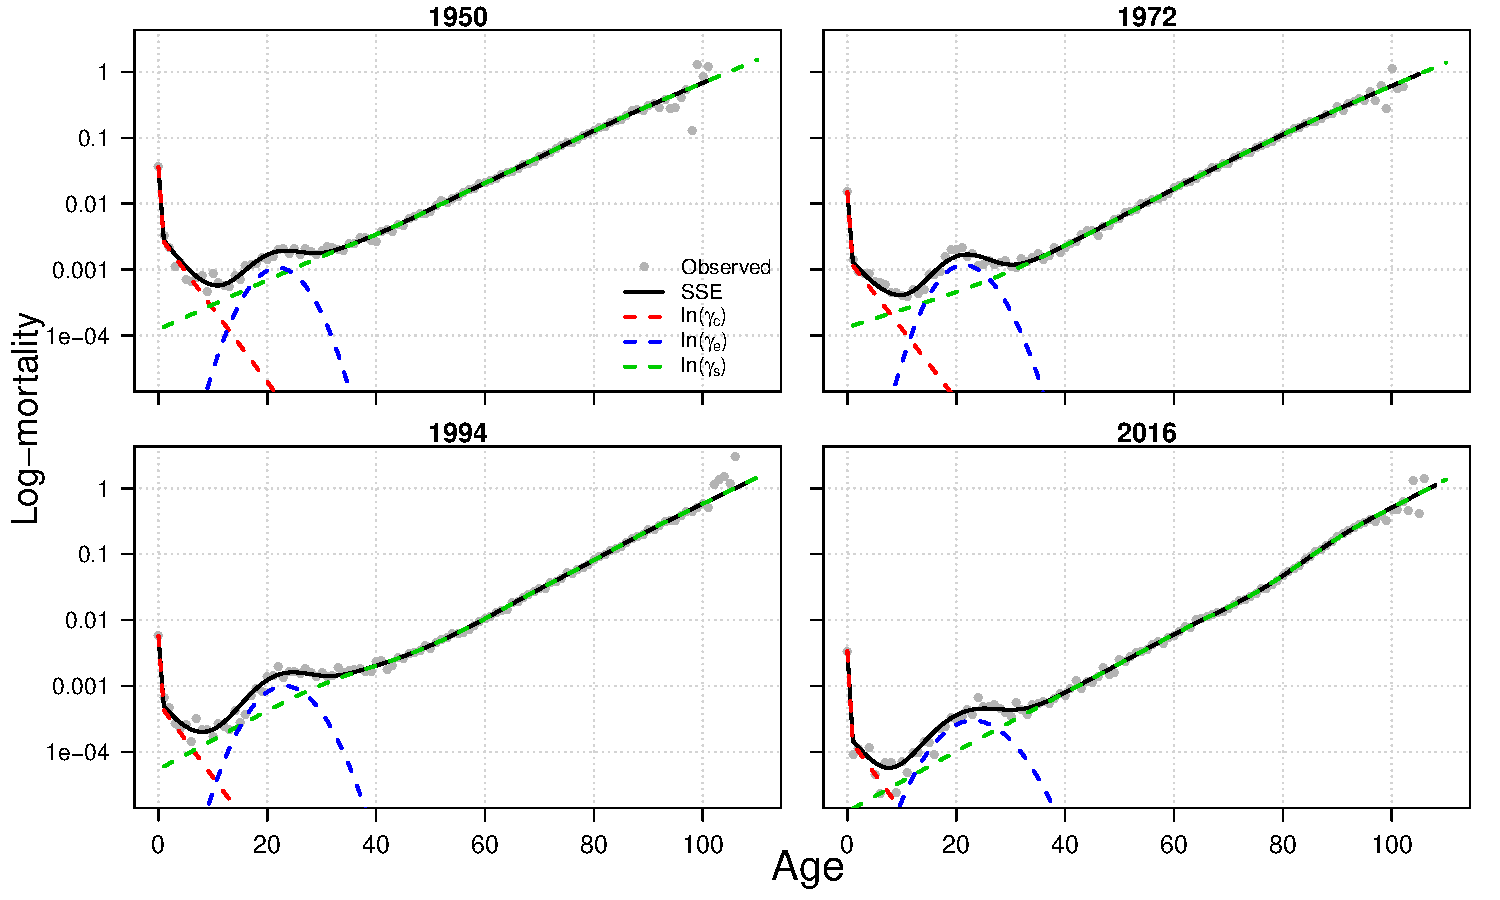
\includegraphics[scale=0.60]{./Ch1/F2.pdf}
		\caption{Evolution of central death rates (on $\log_{10}$ scale, left panel) and age-at-death distributions (right panel) for Swedish females during 1950--2017.\\
		\textit{Source}: Own elaborations based on data from the \cite{HMD}.}\label{Fig:Ch1MxDx}
	\end{center}
\end{figure} 

Age-at-death distributions provide a different yet informative perspective on mortality developments that cannot be directly inferred from the analysis of mortality rates. The right panel of Figure~\ref{Fig:Ch1MxDx} shows the evolution of the age-at-death distributions corresponding to the rates shown in the left panel. The shifting and compression dynamics of mortality captured by the location--scale family (Cf.~Chapter~\ref{Ch2}) are detectable from the changes in the age-at-death distribution. Specifically, the graphs clearly show the shift of the distribution towards older ages, accompanied by a decrease in the overall variability. 

As such, age-at-death distributions are perfectly placed to answer two key questions in mortality studies: (Q1) how long do we live on average? and (Q2) how variable is the age at which we die? \citep{ouellette2011changes}. Indeed, the distribution of deaths provides key insights on the "central longevity indicators" \cite[mean, median and modal age at death,][Q1]{cheung2005three,canudas2010three}, as well as on the variability of lifespans (Q2), an area of research that has recently received increasing attention due to its relevant implications for public health \citep{vanraalte2018case}. As a consequence, the distribution of deaths has been subject to increasing interest in mortality analysis during the most recent years \cite[see, e.g.,][]{ouellette2011changes,mazzuco2018mortality,keilman2019mortality}. 

Despite being well suited to analysing mortality developments, only a few efforts have been made to leverage age-at-death distributions for modelling and forecasting mortality \cite[see, e.g.,][]{oeppen2008coherent,oeppen2013coherent,bergeron2017coherent,pascariu2019maximum}. For these reasons, Chapter \ref{Ch3} introduces an age-at-death distribution model to forecast adult mortality. The proposed approach is a relational model, where a time-unvarying standard (or reference) distribution is transformed over time to capture the observed mortality changes. The transformation takes the form of a segmented linear function, hence we denote the model Segmented Transformation Age-at-death Distributions (STAD). The STAD model is parsimonious and efficient: its three parameters allow us to successfully capture adult mortality developments over age and time, and to disentangle the shifting and compression dynamics of mortality change. Moreover, mortality forecasts can be derived from the extrapolation of the three parameters using standard time-series models.

In the context of projecting mortality in high-longevity countries, the STAD point forecasts are generally more accurate than those of the benchmark \cite{lee1992modeling} model and its extensions, and STAD prediction intervals are well calibrated. Furthermore, STAD forecasts until 2040 are more optimistic and characterized by stronger shifts and smaller compression than those of the methodologies based on mortality rates.

\section{Ch.~\ref{Ch4}: modelling and forecasting age-at-death distributions}\label{Sec:Ch1sec7}
Demographers are generally interested in mortality patterns comprising the full age range. Knowledge of the entire mortality curve is required to derive widely used summary measures that are not conditioned upon surviving to some ages. For example, life expectancy at birth can only be computed when mortality data are available at all ages. 

As such, it is desirable to extend the STAD methodology to produce forecasts for the entire mortality pattern. This is not a straightforward task: using the STAD model (cf.~Chapter \ref{Ch3}) from age 0 instead of age 30 significantly reduces fitting and forecasting accuracy. The reason for this lies in the shape of the human mortality pattern. Since the seminal contribution of \cite{thiele1871mathematical}, demographers decompose the mortality age-profile into three different groups operating principally, or almost exclusively, upon juvenile, younger adult and older adult ages. The STAD model is specifically designed to study and forecast the Senescent component of mortality (i.e.~mortality from age 30 onwards), and a plain extrapolation of the standard distribution disregards the first two mortality components, resulting in a loss of accuracy.    

Chapter~\ref{Ch4} proposes a two-step approach to forecast mortality at all ages using age-at-death distributions and the STAD framework. The procedure is based on: (i) a non-parametric decomposition of the mortality pattern into three independent components corresponding to Childhood, Early-Adulthood and Senescence, respectively, and (ii) modelling and forecasting changes in the three component-specific distributions using specialized versions of the STAD. As such, we call our model Three-Component Segmented Transformation Age-at-death Distributions (3C-STAD). Overall mortality developments are obtained by combining the three components, and mortality forecasts are derived from parameters' extrapolation using standard time series models.  

We compare forecasts of the 3C-STAD model with those of three other well-known approaches to forecasting mortality in two high-longevity countries by sex. The 3C-STAD forecasts generally outperform those of other models, as they are more accurate in terms of both point forecasts and prediction intervals. In addition to this, three main findings emerge from forecasting mortality until 2050: (i)  the 3C-STAD model forecasts more optimistic longevity improvements than approaches based on mortality rates, (ii) projected mortality schedules of the 3C-STAD are smooth, lacking the jaggedness and irregularities found in other models, and (iii) the 3C-STAD forecast age-at-death distributions are characterized by greater shift and less compression than those of other approaches.

\section{Ch.~\ref{Ch5}: forecasting cohort age-at-death distributions}\label{Sec:Ch1sec8}
In addition to being based on central death rates, a second common characteristic of the recently proposed approaches to forecast mortality (cf.~Section~\ref{Sec:Ch1sec3}) is that they focus on the age-period perspective, i.e.~the goal of the model is to forecast mortality patterns in future years. A different approach to mortality forecasting, which has been largely overlooked and unexplored in the actuarial and demographic literature, consists in shifting from the age-period to the age-cohort perspective: here, the goal of the model is the completion of the mortality experience of non-extinct (i.e.~partially observed) cohorts. 

Models to forecast cohort mortality are rather few in the literature: three models have been recently proposed with this explicit purpose \citep{chiou2009modeling,zanotto2017reconstruction,rizzi2019forecasting}, and the 2D $P$-spline of \cite{currie2004smoothing} has been used for completing cohorts in England \& Wales \citep{cmi2007stochastic}. The main reason for the scarcity of efforts in this direction is the heavy data demands that such models require. However, this issue is reduced when the analysis is restricted to adult mortality \citep{booth2006demographic}.

Nonetheless, completing the mortality experience of partially observed cohorts is often an important goal for insurance companies, which are typically interested in the mortality developments of clients born in different cohorts. In such cases, cohort projections are obtained by first forecasting mortality in a period fashion, and then by extracting the cohort patterns from the diagonals of the forecast Lexis surface. Despite being widely used, this approach seems rather counter-intuitive and inefficient, and it can generate implausible prediction intervals \citep{vanraalte2018lifespan}. 

Furthermore, analyses of cohort mortality have an important advantage over those based on the period perspective. Cohort mortality developments are actually observed, whereas period ones are based on the assumption of unchanged mortality rates intrinsic to (period) life tables. Survival in real birth cohorts may thus differ from survival in the hypothetical situation of constant mortality rates because of: (i) tempo effects, (ii) cohort effects and (iii) selection \cite[for a full discussion, see][pp.~90--92]{borgan2019cohort}. Indeed, analyses of age-cohort data have provided different insights into mortality developments than studies based on the age-period perspective \cite[see, e.g.,][]{goldstein2006relationships,shkolnikov2011steep,borgan2019cohort,keilman2019mortality,nepomuceno2019cohort}.

Chapter~\ref{Ch5} contributes a novel methodology to forecast mortality from the age-cohort perspective. The approach is based on adult age-at-death distributions and a generalization of STAD framework (cf.~Chapter \ref{Ch3}). As such, we denote our proposed model Cohort Segmented Transformation Age-at-death Distributions (C-STAD). Unlike the case of age-period data, the original STAD model does not provide a reasonable fit to adult cohort mortality. The main reason is the significant reduction of young adult mortality during the period analysed (cf.~Subsection~\ref{Subsec:Ch5subsec3.2}), mostly due to improvements in sanitary environment, public hygiene and nutrition \citep{mckeown1976modern}. However, the generalization of the segmented transformation of the STAD provides an efficient solution to improve the goodness-of-fit of the C-STAD model.

Our analyses show that the C-STAD is able to successfully capture mortality developments across ages and cohorts, and that it can precisely complete the mortality experience of partially observed cohorts. Specifically, the C-STAD methodology is more accurate than: (i) the 2D $P$-spline model applied to age-cohort data, and (ii) the conventional approach of forecasting age-period mortality with the \cite{lee1992modeling} model, and then extracting cohort patterns from the projected Lexis surface.

\section{Ch.~\ref{Ch6}: smoothing, decomposing and forecasting mortality rates}\label{Sec:Ch1sec9}
In the last chapter of this dissertation, we propose another methodology to model and forecast the entire pattern of mortality from the conventional age-period perspective. Unlike Chapter~\ref{Ch4}, here we adopt the standard approach encountered in the literature, i.e.~we model and forecast central death rates.

Despite its limitations, the seminal model of \cite{lee1992modeling} has been widely adopted by international agencies and private companies, making it the most used mortality forecasting model of modern times. As more thoroughly discussed in Section~\ref{Sec:Ch1sec3}, the three main shortcomings of the model are: (i) the assumption of normality for the error terms, (ii) the jaggedness of the fitted and forecast mortality rates, and (iii) the assumption of a constant rate of age-specific mortality improvements over time. The numerous extensions of the LC model introduced in recent years have been proposed to deal with one drawback at a time. However, none of them addressed these limitations altogether. 

In Chapter~\ref{Ch6}, we propose a generalization of the LC model that captures the complex nature of the mortality age-pattern and simultaneously overcomes the limitations highlighted in the literature. Specifically, the proposed approach: (i) is framed within a Poisson setting; (ii) enforces smoothness in the model parameters, and hence in the outcomes, and (iii) addresses the drawback of the fixed rate of mortality improvement by decomposing mortality into Childhood, Early-Adulthood and Senescent components. Each component is modelled and simultaneously estimated with a smooth variant of the LC model. We hence denote our approach Three-Component smooth Lee-Carter (3C-sLC) model. 

We present the results of fitting and forecasting mortality with the 3C-sLC in four populations, and we compare the outcomes with those obtained from a smooth improved version of the Lee-Carter (LC) model. These analyses show that the 3C-sLC fits the observed mortality data better than the smooth LC model. The increased goodness-of-fit is a direct consequence of the mortality decomposition intrinsic to our proposed approach: mortality developments of the 3C-sLC are described by the combination of the three sets of component-specific LC parameters, which enhance the power and flexibility of the model. 

Moreover, the increased flexibility of the 3C-sLC translates into wider prediction intervals. This is a desirable outcome that directly addresses the criticized narrowness of the LC prediction intervals \citep{alho1992comment}. Finally, specific knowledge on forecast patterns of mortality allows us to perform hypothetical exercises, such as estimating the potential gains in life expectancy derived from the elimination of one or more mortality components.

\section{Discussion \& Outlook}\label{Sec:Ch1sec10}
Despite having a long history in demographic and actuarial analysis, mortality modelling and forecasting is still a very active area of research. Numerous models have been recently proposed to study and project mortality developments over age and time. While significant advances have been made, there still is room for improvement: academics and practitioners are far from achieving a consensus on the most appropriate way to model and forecast human mortality. In addition, currently and widely used forecasting approaches have repeatedly failed to anticipate the sustained rate of mortality improvements observed in many low-mortality countries, generating enormous liabilities for public and private sectors.

The goal of this dissertation was to provide a contribution to the literature on mortality modelling and forecasting by proposing new statistical approaches that can bring novel insights to the analysis of mortality developments. Specifically, the five papers that comprise this thesis directly address the four research questions outlined in Section \ref{Sec:Ch1sec4}, namely: (i) propose a general framework for modelling human mortality, (ii) develop a novel paradigm to forecast mortality that is based on age-at-death distributions, (iii) investigate the unexplored age-cohort dimension in mortality forecasting, and (iv) include the decomposition perspective into mortality forecasting.  

Studies on mortality developments for large populations are generally based on age-specific death rates. Among others, one of the main reasons for this "rate-centric" perspective is that mortality rates easily allow one to capture the change in the risk of death over age, due to their conditioning on the survivors to this particular age \citep{camarda2008smoothing}. As a consequence, the historical development of mortality laws has focused on the force of mortality, i.e.~the continuous counterpart of mortality rates. 

The location--scale (LS) family of models proposed in Chapter \ref{Ch2} reconciles several of these traditional laws of mortality within a unique framework, and it offers desirable properties with respect to their traditional parameterization. Clearly, the LS family is not omni-comprehensive: several existing laws fall outside the scope of the family, whose focus is restricted to the adult mortality pattern. However, the family provides researchers with a new flexible tool for modelling mortality patterns and studying mortality dynamics, and it elegantly joins several laws of mortality within a common framework.

A by-product of the rate-centric perspective discussed is that age-at-death distributions have been neglected for forecasting the future course of mortality. This is rather surprising, because the distribution of deaths provides meaningful demographic insights on mortality developments. The STAD model and its 3C-STAD extension, covered in Chapters \ref{Ch3} and \ref{Ch4}, develop a novel paradigm whereby mortality forecasting is based on age-at-death distributions. These models enlarge the toolbox of demographers, actuaries and, more generally, researchers interested in mortality projections for specific populations. 

A very recent study has shown that the choice of different life-table functions impacts the resulting forecasts, as modelling rates and probabilities of death leads to more pessimistic forecasts than using survival probabilities, life-table deaths and life expectancy \citep{bergeron2019impact}. This is consistent with our findings: forecasts based on the STAD methodology and its extensions are more optimistic than those based on the \cite{lee1992modeling} model and its variants.

Chapter \ref{Ch5} investigates a second unexplored territory in mortality projections, namely cohort mortality forecasting. Cohort forecasts of mortality are interesting for practical purposes: completing the survival experience of partially observed cohorts allows researchers to anticipate demographic developments of real birth cohorts, whose mortality is actually observed and not based on the assumption of constant mortality rates (as for synthetic cohorts of period life tables). Studies of cohort mortality are indeed widespread in the literature, and actuaries are often interested in mortality forecasts of specific cohorts. As such, the proposed C-STAD model can benefit the academic and research community with one of the few approaches to forecasting age-cohort mortality data.

Finally, Chapter \ref{Ch6} proposes a novel extension of the seminal and widely employed \cite{lee1992modeling} model that overcomes its principal limitations. This approach, as well as the 3C-STAD model of Chapter \ref{Ch4}, introduces a highly innovative perspective into mortality forecasts, namely the decomposition of the mortality pattern into three independent components: Childhood, Early-Adulthood and Senescent mortality. Forecast trends can therefore be analysed in terms of these components: for example, it is possible to decompose longevity increases into the contribution of each component.  

Despite the significant advances achieved in mortality forecasting, European demographic forecasts have not become more accurate over the most recent years \citep{keilman2008european}. Although forecasts in the social sciences are unlikely to be as accurate as those in the physical sciences, better separation of signals from noise can lead to improvements in forecast accuracy \citep{makridakis2019forecasting}. The methods proposed in this thesis are a step in this direction: forecasts obtained with the STAD, 3C-STAD and C-STAD models have been shown to produce more accurate point forecasts than other projection methodologies in several out-of-sample validation exercises.

A second important aspect of forecasting concerns prediction intervals. Until recently, little attention was paid to forecast distributions, or measures of forecast distribution accuracy  \citep{makridakis2019forecasting}. However, the uncertainty surrounding point forecasts is equally important as the point forecast itself.  Prediction intervals indeed allow for a more thorough comparison of different forecasting methodologies \citep{chatfield2000time}. This feature is often neglected in the demographic literature, where the focus is generally restricted to point forecast accuracy. In Chapters \ref{Ch3} and \ref{Ch4}, we assessed and compared the prediction interval accuracy of the STAD and 3C-STAD models, finding increased precision when compared to the more traditional forecasting approaches. As such, this dissertation stimulates the consideration of this important procedure. 

Several directions of future research can currently be foreseen. Despite enabling reproducibility and implementation of the routines developed in this thesis (cf.~Section~\ref{Sec:Ch1sec11}), a freely available \texttt{R} package \citep{Rcite} in the Comprehensive \texttt{R} Archive Network (CRAN) would allow researchers to more easily employ the methodologies presented in this dissertation. The development of such package is planned for future work.

In light of the recent efforts towards the production of coherent forecasts for multiple (sub)-populations, the STAD framework could be extended to achieve this goal. For example, a coherent standard distribution could be derived from combining the mortality experience of different populations, and the population-specific parameters could be forecast within a multivariate time-series setting. This would allow one to include coherence as an additional factor in age-at-death distribution forecasts.

Furthermore, the STAD methodology could be enlarged outside the analysis of all-cause mortality. Cause-specific age-at-death distributions could be analysed and forecast with the STAD model or its modifications. For example, it could be possible to distinguish between smoking and non-smoking related mortality, as in \cite{janssen2013smoking}. In addition to this, fertility and migration data could be analysed and forecast with adaptations of the STAD approach.

Finally, one limitation of the 3C-STAD and C-STAD models that could benefit from future work concerns computation speed. Generating results from the two models, specifically the prediction intervals, requires more time than other widespread forecasting approaches. Increased computer power will accelerate these procedures, but more specific solutions could be developed.

\section{Reproducibility}\label{Sec:Ch1sec11}
All manuscripts of the thesis have been written with the goal of complying to the good practices of open science, namely code sharing and reproducibility of results. Routines for implementing the models presented in this thesis, which have all been developed in the free \texttt{R} software \citep{Rcite}, are already available online for the articles that have been published and accepted for publication, and they will be made public upon eventual acceptance of the two manuscripts under review. 

Specifically, routines for fitting the location-scale (LS) family of models presented in Chapter \ref{Ch2} can be found at  \url{https://github.com/ubasellini/LocationScale}, or in the Supplementary Material of the published article (\url{ https://doi.org/10.1007/s10680-018-9497-x}). The available codes readily allow one to estimate the location and scale parameters for any HMD population as well as for the eleven models belonging to the LS family.

Modelling and forecasting mortality with the Segmented Transformation Age-at-death Distributions (STAD) model introduced in Chapter \ref{Ch3} can be readily performed using the codes provided at \url{https://github.com/ubasellini/ForecastingDistributions}, or in the Supplementary Material of the published article (\url{https://www.tandfonline.com/doi/full/10.1080/00324728.2018.1545918}).

The generalisation of the STAD model to the entire age range, i.e.~the Three-Component STAD (3C-STAD) model presented in Chapter~\ref{Ch4}, can be implemented with the routines available at \url{https://github.com/ubasellini/3C-STADmodel}. Furthermore, this GitHub repository contains all the results presented in the final accepted version of the book chapter.

Moreover, routines and results derived from the Cohort STAD (C-STAD) model of Chapter \ref{Ch5} are placed in the GitHub repository \url{https://github.com/ubasellini/C-STAD}, which is currently private (i.e.~accessible only to collaborators) to comply with the guidelines of the journal where the manuscript is under review. Nonetheless, the repository will be made publicly available upon eventual acceptance of the manuscript. 

Finally, routines for smoothing, decomposing and forecasting mortality with the Three-Component smooth Lee-Carter (3C-sLC) model of Chapter \ref{Ch6} are available at \url{https://osf.io/rgf8y/?view_only=1608f0f8d1e9466cb33733bb03057b80}. This is a freely accessible open science framework link, which we have made anonymous for peer review of the manuscript. 

\cleardoublepage

\end{document}